\documentclass{beamer}
\def\presentationtype{0}
\def\corsodilaurea{Ingegneria Informatica e dell'Automazione Industriale}
\def\insegnamento{Ottimizzazione}
\def\nolezione{8}
\def\titolo{Il metodo del simplesso -- Il ``tableau'' e l'operazione ``pivot''}
\def\noattivita{1}

\def\argomenti{Programmazione Lineare}
\def\obiettivilezione{Definire il ``tableau'' e l'operazione ``pivot'' per poter sviluppare metodo del simplesso primale}
\def\nucleotematico{Richiami}
\def\contenuto{Programmazione lineare}


\usepackage[italian]{babel}
%
% Hyperref info for PDF
%
\usepackage{hyperref}
\hypersetup{%
%pdfpagemode=FullScreen,
pdfpagemode=FullScreen,
pdfstartview=Fit,
pdfsubject={\argomenti},
pdfkeywords={\insegnamento,\titolo}
}

\definecolor{ecampus@engred}{RGB}{227,28,23}
\setbeamercolor{normal text}{fg=black,bg=}
\setbeamercolor{alerted text}{fg=red}
\setbeamercolor{example text}{fg=green!50!black}
\setbeamercolor{structure}{fg=ecampus@engred,bg=}
\usetheme{default}
\useinnertheme{rounded}%{circles}
\setbeamertemplate{blocks}[default]
\setbeamercolor{block title}{bg=}
\setbeamercolor{block body}{bg=}

\ifnum\presentationtype>0 {\setbeamertemplate{enumerate item}{Es. \nolezione.\presentationtype.\arabic{enumi})}} \fi

%\setbeamertemplate{frametitle continuation}[from second][(cont'd)]
\usefonttheme[stillsansseriftext,stillsansserifsmall]{serif}
\setbeamertemplate{headline}{%
\leavevmode%
   \hspace*{4.75cm}
   \scalebox{0.90}{%
    \begin{minipage}{\linewidth}%
      \tiny
 	\begin{tabular}{ll}
	  \\
% 	  \textcolor{gray}{Classe}					& \corsodilaurea\\
%	  \textcolor{gray}{Argomento:}					& \insegnamento\\
%	  \textcolor{gray}{Lezione n}:							& \nolezione \\
	  \textcolor{gray}{Titolo:}			& \titolo \\
	  \textcolor{gray}{Attivit\`a}:		& 	  \ifnum\presentationtype=0 {Lezione \nolezione} \else {Sessione di studio \nolezione.\presentationtype} \fi
	\end{tabular}%
    \end{minipage}%
   }%
}
\setbeamertemplate{footline}[text line]{%
  \begin{minipage}{\linewidth}%
    \hfill\insertpagenumber%
%    
    \begin{center}%
      \rule{\linewidth}{0.4pt}
    \end{center}
    \vspace*{-0.65cm}
    \begin{center}%
      \scalebox{0.55}{%
	\begin{minipage}{\linewidth}%
	  \begin{center}%
	    {\tiny
	    \copyright \ 2022 Gionata Massi - \color{blue}{\href{mailto:gionata.massi@savoiabenincasa.it}{gionata.massi@savoiabenincasa.it}}\\
	    \phantom{XXX}}
	  \end{center}
	\end{minipage}%
      }%
    \end{center}%
%
  \end{minipage}%
  }
\setbeamertemplate{navigation symbols}{}

%% Save up on ink for the 4-up handouts
\mode<handout>{%
  \pgfpagesuselayout{4 on 1}[a4paper, landscape, border shrink=10mm]
  \pgfpageslogicalpageoptions{1}{border code=\pgfstroke}
  \pgfpageslogicalpageoptions{2}{border code=\pgfstroke}
  \pgfpageslogicalpageoptions{3}{border code=\pgfstroke}
  \pgfpageslogicalpageoptions{4}{border code=\pgfstroke}
}

\mode<presentation>{\AtBeginSection{%
  \begin{frame}
    \frametitle{Piano della presentazione}
    \tableofcontents[currentsection]
  \end{frame}}
}

\usepackage{microtype}
\usepackage[utf8]{inputenc}
\usepackage[T1]{fontenc}
%\usepackage[osfss]{libertine}
\usepackage{palatino}
\usepackage[scaled=.77]{beramono}
\usepackage{booktabs}
% \usepackage{attachfile}

% Toglie l'enorme spazione prima di description
%\setbeamersize{description width=0pt}

\usepackage{tikz}
\usetikzlibrary{decorations,arrows,shapes,backgrounds,matrix,positioning}
\usepackage{multirow}
\usepackage{verbatim}
\usepackage{eurosym}
\usepackage{pgfpages}

\usepackage{zref-savepos}
\newcounter{restofframe}
\newsavebox{\restofframebox}
\newlength{\mylowermargin}
\setlength{\mylowermargin}{2pt}

\newenvironment{restofframe}{%
    \par%\centering
    \stepcounter{restofframe}%
    \zsavepos{restofframe-\arabic{restofframe}-begin}%
    \begin{lrbox}{\restofframebox}%
}{%
    \end{lrbox}%
    \setkeys{Gin}{keepaspectratio}%
    \raisebox{\dimexpr-\height+\ht\strutbox\relax}[0pt][0pt]{%
    \resizebox*{!}{\dimexpr\zposy{restofframe-\arabic{restofframe}-begin}sp-\zposy{restofframe-\arabic{restofframe}-end}sp-\mylowermargin\relax}%
        {\usebox{\restofframebox}}%
    }%
    \vskip0pt plus 1filll\relax
    \mbox{\zsavepos{restofframe-\arabic{restofframe}-end}}%
    \par
}

\title{\titolo}
\author{Gionata Massi}
\date{\today}

\setbeamercolor*{frametitle}{fg=black}
\setbeamercolor*{title}{fg=black}
\setbeamerfont{frametitle}{shape=\scshape,family=\rmfamily,size=\large,series=\bfseries}

\setbeamersize{}
\makeatletter
\newcommand\thefontsize[1]{{#1 The current font size is: \f@size pt\par}}
\makeatother

\tikzstyle{nicebox}=[draw=gray!100, fill=blue!10, very thick,
rounded corners, rectangle, inner sep=4pt, inner ysep=16pt]
\tikzstyle{niceboxtitle}=[draw=gray!100, fill=white, text=black,
rounded corners, very thick, rectangle]
\newcommand\nicebox[2]{
{\centering
\begin{tikzpicture}
\node [nicebox](box){
\begin{minipage}{0.95\textwidth}\centering
\begin{minipage}{0.95\textwidth}
#2
\end{minipage}\end{minipage}};
\node[niceboxtitle, right=10pt] at (box.north west)
{\small\textbf{#1}};
\end{tikzpicture}\par}
}

\tikzstyle{modelbox}=[draw=structure!100, fill=white!50, very thick,
rounded corners, rectangle, inner sep=4pt, inner ysep=16pt, text=blue!50!black]
\tikzstyle{modelboxtitle}=[draw=structure!100, fill=white!50, text=blue!50!black,
rounded corners, very thick, rectangle]
\newcommand\modelbox[2]{
{\centering
\begin{tikzpicture}
\node [modelbox](box){
\begin{minipage}{0.95\textwidth}\centering
\begin{minipage}{0.95\textwidth}
#2
\end{minipage}\end{minipage}};
\node[modelboxtitle, right=10pt] at (box.north west)
{\small\textbf{\mbox{#1}}};
\end{tikzpicture}\par}
}

% % %
% Tipi di sessioni di studio
% % %
\def\domande{Domande}
\def\approfondimenti{Approfondimenti}
\def\esercizi{Esercizi}
\def\esempi{Esempi svolti}
\def\relazioni{Relazioni}
\def\attivitapratica{Attivit\`a pratica}
% % %

\newcommand{\generatitolo}{ %
\begin{frame}[plain]
\pdfbookmark{\ifnum\presentationtype=0 {Lezione \nolezione} \else {Sessione di studio \nolezione.\presentationtype} \fi}{\ifnum\presentationtype=0 {Lezione \nolezione} \else {Sessione di studio \nolezione.\presentationtype} \fi}
\noindent\hspace*{3.715cm}
   \scalebox{0.90}{%
    \begin{minipage}{\linewidth}%
      \tiny
 	\begin{tabular}{ll}
	  \\
% 	  \textcolor{gray}{Classe}					& \corsodilaurea\\
%	  \textcolor{gray}{Argomento:}					& \insegnamento\\
%	  \textcolor{gray}{Lezione n}:							& \nolezione \\
	  \textcolor{gray}{Titolo:}			& \titolo \\
	  \textcolor{gray}{Attivit\`a}:		& 	  \ifnum\presentationtype=0 {Lezione \nolezione} \else {Sessione di studio \nolezione.\presentationtype} \fi
	\end{tabular}%
    \end{minipage}%
   }%
   
  \begin{center}
    \large{\textbf{\insegnamento}}
  \end{center}

  \vspace*{0.5cm}
  
  \begin{center}
    \huge{\titolo}
  \end{center}
  
  \begin{center}
	  \ifnum\presentationtype=0
	    {Lezione n$^{\circ}$ \nolezione}
	  \else
	    {Sessione di studio n$^{\circ}$ \nolezione .\presentationtype}
	  \fi
  \end{center}
  
  \vspace*{0.5cm}

  \begin{center}
    \large{\textsl{Gionata Massi}}\\
    \scriptsize\color{blue}{<\href{mailto:gionata.massi@savoiabenincasa.it}{gionata.massi@savoiabenincasa.it}>}
  \end{center}
  
  \newcounter{pageleft}
  \zsaveposy{pageleft}
  \vspace*{\dimexpr\zposy{pageleft}sp-1.67cm}

  \begin{minipage}{\linewidth}%
   \hfill\phantom{\insertpagenumber}%

  \begin{center}%
      \rule{\linewidth}{0.4pt}
    \end{center}
    
    \vspace*{-0.95cm}
    
    \begin{center}%
      \scalebox{0.55}{%
	\begin{minipage}{\linewidth}%
	  %\begin{center}%
	  %  \tiny
	  %  \copyright \ 2022 Gionata Massi - \color{blue}{\href{mailto:gionata.massi@savoiabenincasa.it}{gionata.massi@savoiabenincasa.it}}\\
	  %  \color{blue}{\href{mailto:gionata.massi@savoiabenincasa.it}{gionata.massi@savoiabenincasa.it}}\\
	  %  \phantom{XXX}
	  %\end{center}
	\end{minipage}%
      }%
    \end{center}%
     \phantom{XXX}
%
  \end{minipage}%

\end{frame}
}

\renewcommand{\vec}{\mathbf}
\newcommand{\matr}{\mathbf}

\uselanguage{italian}
\languagepath{italian}
\deftranslation[to=italian]{Theorem}{Teorema}
\deftranslation[to=italian]{theorem}{teorema}
\deftranslation[to=italian]{Definition}{Definizione}
\deftranslation[to=italian]{definition}{definizione}
\deftranslation[to=italian]{Corollary}{Corollario}
\deftranslation[to=italian]{corollary}{corollario}

\let\definition\relax
\let\enddefinition\relax

%\theoremstyle{example}
\newtheorem{definition}[theorem]{\translate{Definition}}

\def\fieldN{\mathbb{N}}
\def\fieldR{\mathbb{R}}
\def\fieldZ{\mathbb{Z}}

\def\matrA{\matr{A}}
\def\vecB{\vec{b}}
\def\vecC{\vec{c}}
\def\vecX{\vec{x}}

\usepackage{cancel}
\usepackage{bookmark}

% tkiz ball item
\newcommand*\circled[1]{\raisebox{2.5pt}{\tikz[baseline=(char.base)]{
            \node[circle,ball color=purple, shade, 
 color=white,inner sep=1.2pt] (char) {\tiny #1};}}}

% tkiz rounded item
\newcommand*\rounded[1]{\tikz[baseline=(char.base)]{
            \node[draw=none,ball color=purple, shade, 
 color=white, rounded corners=3.5pt, inner sep=2.5pt] (char) {\scriptsize #1};}}

 \usepackage{etoolbox}
\makeatletter
\apptocmd{\beamer@@frametitle}{\write\@auxout{\string\@writefile{frm}{\string\frametitleentry{\the\c@framenumber}{#1}{#2}}}}{}{}
\newcommand*{\frametitleentry}[3]{\@namedef{frametitleshort#1}{#2}\@namedef{frametitle#1}{#3}}
\AtEndDocument{\if@filesw\newwrite\tf@frm\immediate\openout\tf@frm\jobname.frm\relax\fi}
\@input{\jobname.frm}
\makeatother
 
%\usebackgroundtemplate{
\includegraphics[width=\paperwidth]{../img/sfondo_ecampus.png}}

\usepackage{listings}
% Extension for listings package
\lstdefinelanguage{ampl}{
  % See AMPL book (1993 edition), Appendix A
  morekeywords={%
    % Table A.1
    % Excluding symbols and "not X", where X (and not) are keywords
    if, then, else, or,  exists, forall,  and, in, within, 
    not, union, diff, symdiff, inter, cross, setof, by, 
    % Skipping: less,  sum, prod, min, max, div, mod,
    % Skipping built-in functions (Tables A-2 and A-3)
    % Section A.5 -- Declarations of model entities (subject to ->
    % subject, to)
    set, param, var, arc, minimize, maximize, subject, to, node,
    % Section A.6 -- Set declarations (not repeating set or within)
    dimen, default, card, ordered, by, reversed, circular,
    % Section A.7 -- Parameter declarations (not repeating in, default)
    param, binary, integer, symbolic, check, Infinity
    % Section A.8 -- Variable declarations
    var,  coeff, cover, obj,
    % Section A.13 -- Command language
    % Skipping most commands!
    include, model, data, let, objective, drop, restore, solve,
    solution, quit, end, option, reset, update, commands,
    % A.14 -- Imported functions
    function, pipe, 
    % A.17 synonyms for previously-defined keywords
    coef, difference, dimen, dimension, intersect, intersection, s.t., 
    % 
    % must be defined somewhere ...
    for, while, repeat, break,
    % NEW language features (http://www.ampl.com/NEW/newlang.html)
    % Grouped by page
    purge, problem, redeclare, xref,
    complements, 
    table, IN, OUT, INOUT, read, write, 
    expand,
    for, commands, repeat, until, while, break, continue,
  },
  sensitive=true,
  comment=[l]{\#},
  morecomment=[s]{/*}{*/},
  string=[b]",
  morestring=[b]',
}[keywords,comments,strings]

\definecolor{comment_c}{RGB}{60,128,49}
\definecolor{rowname_c}{RGB}{128,60,49}
\definecolor{reserved_c}{RGB}{49,60,128}

\lstset{
	language=ampl,%
	commentstyle=\color{comment_c},%
	backgroundcolor=\color{blue!15},%
    basicstyle=\small\ttfamily,%
    %emph={s.t.},emphstyle={\bfseries},%
    otherkeywords={s.t.},%
    numbers=left, numberstyle=\tiny, stepnumber=1, numbersep=5pt,%
}

\definecolor{col_set}{RGB}{128,0,0}
\definecolor{col_par}{RGB}{91,0,91}
\definecolor{col_idx}{RGB}{0,91,91}
\definecolor{col_var}{RGB}{0,0,128}

\def\insieme{%1}{\rm \textcolor{col_set}{%1}}}


\begin{document}

\generatitolo

\section{Analisi post-ottimale}

\begin{frame}{Analisi di post-ottimalit\`a}
  \begin{itemize}
  \item La determinazione di una soluzione ottima di un problema di programmazione
  lineare non completa l'analisi da compiere sul modello matematico
  (e sul problema in esame)
  %in quanto dalla soluzione del modello possono essere
  %estratte informazioni aggiuntive

  \item L'analisi di post-ottimalit\`a (detta anche di sensitività) ha lo scopo di
  verificare entro quali limiti la soluzione ottima trovata resta invariata se
  vengono modificati alcuni parametri del problema

  \item Quando un problema di P.L. presenta due variabili decisionali è possibile
  impiegare un metodo di analisi di post-ottimalità basato su considerazioni
  geometriche e rappresentabile graficamente sul piano cartesiano $Ox_1x_2$
  \end{itemize}
\end{frame}

\section{Programma lineare di esempio}

\begin{frame}[allowframebreaks]{Problema di esempio}
\fontsize{7}{8.4}{
\begin{block}{Mix ottimo di produzione}
Un'azienda di produzione vuole determinare il tasso di produzione mensile di due prodotti
in modo da massimizzare il profitto netto totale,  sapendo che:
 \begin{itemize}
  \item per produrre un quintale di prodotto 1 occorrono 40 quintali di materia prima e 8 ore di lavoro;
  \item per produrre un quintale di prodotto 2 occorrono 20 quintali di materia prima e 2 ore di lavoro;
  \item il commerciale ha stabilito che la produzione totale mensile non pu\`o superare 100 quintali;
  \item la disponibilità mensile di materia prima \`e di 2200 quintali e quella di lavoro di 320 ore;
  \item il profitto netto per la vendita dei prodotti 1 e 2 sia rispettivamente 120 e 40 euro.
 \end{itemize}
\end{block}
}

\framebreak

\modelbox{Modello}{%
\small{%
$$\begin{array}{crrrlcr}
\max z=& 120 x_1 &+& 40 x_2    &           & (0) & [\text{profitto}]\\
{\rm s.t.} & 40 x_1 &+& 20 x_2 & \leq 2200 & (1) & [\text{materie prime}]\\
           &  8 x_1 &+&  2 x_2 & \leq 320  & (2) & [\text{lavoro}]\\
           &    x_1 &+&    x_2 & \leq 100  & (3) & [\text{mercato}]\\
           \multicolumn{5}{c}{x_1 \geq 0,\ x_2 \geq 0} & & [\text{non negativit\`a}]
\end{array}$$}}


\end{frame}

\begin{frame}{Soluzione ottima}
\centering
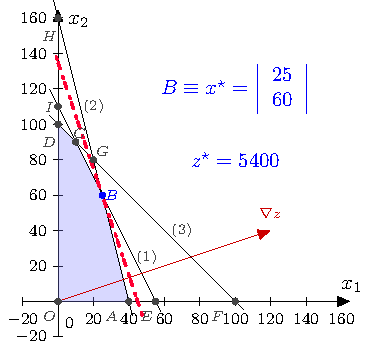
\includegraphics{img/mix_ottimo_sol}
\end{frame}

\section{Analisi delle risorse}

\begin{frame}{Variazioni del valore dei parametri}
\begin{itemize}
\item 
  Nel problema di produzione \`e interessante conoscere come
  sono utilizzate le risorse disponibili,
  in particolare capire se:
  \begin{itemize}
  \item 
  si possono avere vantaggi da un aumento della loro disponibilit\`a,
  \item 
  si può diminuire la loro disponibilit\`a senza modificare il valore ottimo dell'obiettivo.
  \end{itemize}
  
  \item \`E, inoltre, interessante capire come cambierebbe la soluzione
  (le quantità ottime di prodotti da realizzare)
  se variassero i prezzi di vendita.
\end{itemize}
\end{frame}

\begin{frame}[allowframebreaks]{Analisi delle risorse}
\begin{itemize}
\item 
  Consideriamo due tipi di variazione rispetto alla disponibilità delle risorse:
  \begin{itemize}
  \item 
  come aumentare le risorse per migliorare la soluzione ottima
  \item 
  come ridurre le risorse disponibili lasciando invariata la soluzione ottima
  \end{itemize}
  
  \item  Notiamo che i vincoli del problema hanno tutti la seguente forma
  \begin{itemize}
  \item quantità di risorsa usata $\leq$ disponibilit\`a di risorsa
  \end{itemize}
  
  \item I vincoli $(1)$ e $(2)$ sono soddisfatti all'uguaglianza dalla soluzione ottima,
  rappresentata dal punto $B$ di coordinate $(25,60)$,

  \item quindi il livello ottimo di produzione per i due prodotti \`e tale da utilizzare
  tutte le materie prime e tutta la disponibilit\`a di lavoro.

  \item I vincoli $(1)$ e $(2)$ si dicono saturi, e le materie prime e la capacità produttiva,
  poich\'e sono utilizzate completamente, si dicono risorse scarse.
  
  \item \`E possibile aumentare la disponibilit\`a di una risorsa scarsa per migliorare
  la soluzione ottima.

  \item \`E possibile diminuire la disponibilità di una risorsa abbondante senza variare
  la soluzione ottima.
\end{itemize}
\end{frame}

\section{Variazione dei termini noti}

\begin{frame}{Analisi delle risorse -- variazioni di $b_1$}
\mbox{\parbox[c][0.8\textheight]{6.8cm}{
 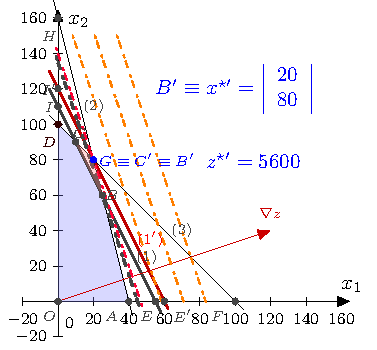
\includegraphics{img/mix_ottimo_b1_2400}}
\parbox[c][0.8\textheight]{4cm}{
   \tiny{%
    Supponiamo di voler aumentare la disponibilità della sola risorsa
    \emph{scarsa} $b_1$ (materia prima) e verifichiamo qual è il
    massimo incremento che ha senso introdurre.

  \vspace*{1em}
  
  Aumentando la risorsa $b_1$ il vincolo (1), saturo nel punto di ottimo,
  trasla parallelamente a se stesso verso  destra e di conseguenza variano la regione
  ammissibile e il punto di ottimo
  
  \vspace*{1em}

  In figura è illustrata la variazione della risorsa da 
  $b_1 = 2200$ a  $b_1^\prime = 2400$
  
  \vspace*{1em}
  
  Oltre $G = (20, 80)$, intersezione di $(2)$ e $(3)$, non ha più senso aumentare $b_1$
  Se si aumentasse ulteriormente la risorsa  b1 non si modificherebbe la regione di 
  ammissibilità.

  Ha senso incrementare  $b_1$ fino a quando tale risorsa è usata completamente,
  in questo caso fino al valore $2400$.
  }}}
\end{frame}

\begin{frame}{Analisi delle risorse -- variazioni di $b_2$}
\mbox{\parbox[c][0.8\textheight]{6.8cm}{
 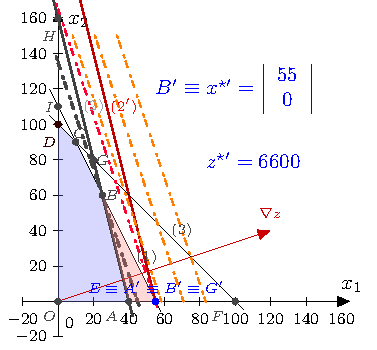
\includegraphics{img/mix_ottimo_b2_440}}
\parbox[c][0.8\textheight]{4cm}{
   \tiny{%
   Si può sviluppare un discorso analogo per variazioni della risorsa scarsa
   $b_2$ (lasciando invariate le altre risorse)

  \vspace*{1em}
  
  Aumentando la risorsa $b_2$ il vincolo (2), saturo nel punto di ottimo,
  trasla parallelamente a se stesso verso destra e di conseguenza variano la regione
  ammissibile e il punto di ottimo
  
  \vspace*{1em}

  In figura è illustrata la variazione della risorsa da 
  $b_2 = 320$ a  $b_2^\prime = 440$
  
  \vspace*{1em}
  
 La nuova soluzione ottima vale 6600 in corrispondenza del punto $E = (55, 0)$.
 
 Aumentando oltre 440 la risorsa $b_2$ questa risorsa non sarebbe più scarsa
 nella soluzione ottima e non cambierebbe il valore dell’ottimo.
 }}}
\end{frame}

\begin{frame}{Analisi delle risorse -- variazioni di $b_3$}
\mbox{\parbox[c][0.8\textheight]{6.8cm}{
 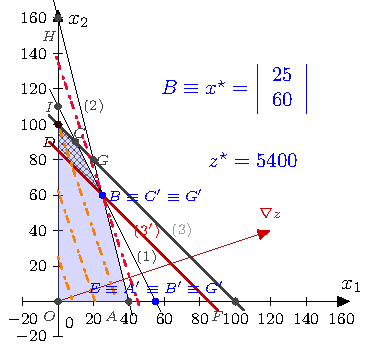
\includegraphics{img/mix_ottimo_b3_85}}
\parbox[c][0.8\textheight]{4cm}{
   \tiny{%
    La risorsa $b_3$ è \emph{abbondante} (non scarsa):
    ci sono delle unità di risorsa in eccedenza che possono essere diminuite,
    entro un certo limite, senza alterare la soluzione ottima
  \vspace*{1em}
  
  All'ottimo si ha un'eccedenza di 15 unità di risorsa $b_3$:
  $x_1 + x_2$ all'ottimo $(25, 60)$ vale 85.

  \vspace*{1em}

   Il vincolo (3), non saturo, può essere traslato parallelamente a se stesso
   verso  sinistra senza che il punto di ottimo esca dalla regione di
   ammissibilità.

  \vspace*{1em}
   
  In figura è illustrata la variazione della risorsa da  $b_3 = 100$
  a  $b_3^\prime = 85$
  
  \vspace*{1em}

  La soluzione ottima non varia.
  }}}
\end{frame}

\section{Valore di una risorsa}

\begin{frame}{Analisi delle risorse}
 Dopo aver verificato la convenienza di una possibile maggiore
 disponibilità delle risorse $b_1$ e $b_2$, è interessante
 determinare quale sia tra le due la risorsa che di più convenga
 aumentare.

 \vspace*{1em}
 
 Nell'esempio, lìazienda potrebbe avere una limitata disponibilità
 finanziaria che vorrebbe far fruttare al meglio, acquisendo
 un'ulteriore quantità di una delle risorse (materia prima o lavoro)
 in modo da incrementare maggiormente i propri profitti.
\end{frame}

\begin{frame}[allowframebreaks]{Valore di una risorsa}

Si può calcolare il valore di una unità di risorsa $y_i$:

\modelbox{Valore della risorsa $i$-esima}{\large{\[y_i=\frac{\partial z}{\partial b_i}\]}}

\framebreak

\small{
Se la variazione della risorsa $i$-esima è sufficientemente piccola
da far si che il punto di ottimo sia intersezione degli stessi
vincoli saturi, allora:}

\modelbox{Valore della risorsa $i$-esima}{\large{\[y_i=\frac{\Delta z}{\Delta b_i}\]}}

\small{
La quantità $y_i$ indica di quanto aumenta l'obiettivo in corrispondenza
dell’acquisizione di un'ulteriore unità di risorsa}

\framebreak

\footnotesize{
Consideriamo le massime variazioni delle risorse e del punto
di ottimo affinché la soluzione sia intersezione degli stessi
vincoli (saturi)

% Il valore di una unità di risorsa $y_1$ è:
\[
y_1=\frac{\Delta z}{\Delta b_1}
   =\frac{5600-5400}{2400-2200}
   =\frac{200}{200}
   =1 [\text{\euro / q}]
\]

% Il valore di una unità di risorsa $y_2$ è:
\[
y_2=\frac{\Delta z}{\Delta b_2}
   =\frac{6600-5400}{440-320}
   =\frac{1200}{120}
   =10 [\text{h / q}]
\]

% Il valore di una unità di risorsa $y_3$ è:
\[
y_3=\frac{\Delta z}{\Delta b_3}
   =\frac{5400-5400}{85-100}
   =-\frac{0}{15}
   =0 [\text{\euro / dim. mercato}]
\]}
\end{frame}

\section{Variazione dei coefficienti della funzione obiettivo}

\begin{frame}[allowframebreaks]{Variazione dei coefficienti della f.o.}
 Analizziamo ora entro quali limiti di tolleranza possono variare
 i prezzi di vendita dei due prodotti senza alterare la soluzione
 ottima (la produzione associata al punto $B$)

 Variando i coefficienti $c_1$ e $c_2$ cambia la pendenza della
 funzione obiettivo

 Le curve di livello della funzione obiettivo sono il fascio di
 rette $c_1 x_1 + c_2 x_2 = k$

 Nel piano cartesiano $Ox_1x_2$ sono rette con coefficiente angolare
 $-\frac{c_1}{c_2}$ e intercetta $\frac{k}{c_2}$

\framebreak

La pendenza della funzione obiettivo è data da $-\frac{c_1}{c_2}$.
Affinché la soluzione ottima rimanga in $B$ tale valore deve essere
compreso fra quelli delle pendenze dei vincoli attivi:

La pendenza del vincolo $(1)$ è $-\frac{a_{11}}{a_{12}}=-\frac{40}{20}=-2$
e quella di $(2)$ è $-\frac{a_{21}}{a_{22}}=-\frac{8}{2}=-4$

\[\implies -4\leq-\frac{c_1}{c_2}\leq -2\]

\framebreak

Se si lascia invariato $c_2$ e si fa variare $c_1$,
il punto $B$ rimane soluzione ottima fino a che la
pendenza della funzione obiettivo diventa uguale a
quella dei vincoli (1) e (2)

\[
\begin{array}{rlrlrlrlrlr}
 -\frac{c_1}{c_2}&=&-\frac{c_1}{40}&=&-2&\text{ pendenza di }(1)&\implies&c_1=80\\	
 -\frac{c_1}{c_2}&=&-\frac{c_1}{40}&=&-4&\text{ pendenza di }(2)&\implies&c_1=160\\
\end{array}
\]

\[\implies  80 \leq c_1 \leq 160 \]

\framebreak

Se si lascia invariato $c_1$ e si fa variare $c_2$:

\[
\begin{array}{rlrlrlrlrlr}
 -\frac{c_1}{c_2}&=&-\frac{120}{c_2}&=&-2&\text{ pendenza di }(1)&\implies&c_2=60\\	
 -\frac{c_1}{c_2}&=&-\frac{120}{c_2}&=&-4&\text{ pendenza di }(2)&\implies&c_2=30\\
\end{array}
\]
\[\implies  30 \leq c_1 \leq 60 \]

\framebreak

\mbox{\parbox[c][0.8\textheight]{6.8cm}{
 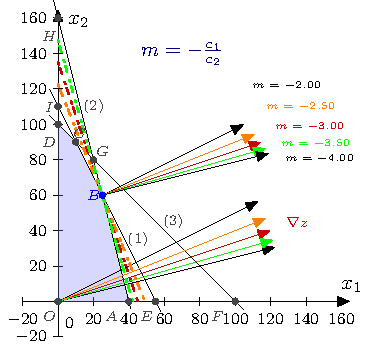
\includegraphics{img/mix_ottimo_var_coeff}}
\parbox[c][0.8\textheight]{4cm}{
   \tiny{%
 Il punto di ottimo rimane $B$ se:

 $80 \leq c_1 \leq 160,\text{ con }c_2 = 40$
 
 $30 \leq c_2 \leq 60,\text{ con }c_1 = 120$
}}}
\end{frame}


\end{document}
